\documentclass[11pt,a4paper]{jsarticle}
%
\usepackage{listings,jlisting}
\usepackage{amsmath,amssymb}
\usepackage{bm}
\usepackage{ascmac}
\usepackage[dvipdfmx]{graphicx}
\usepackage{here}
%ここからソースコードの表示に関する設定
\lstset{
  basicstyle={\ttfamily},
  identifierstyle={\small},
  commentstyle={\smallitshape},
  keywordstyle={\small\bfseries},
  ndkeywordstyle={\small},
  stringstyle={\small\ttfamily},
  frame={tb},
  breaklines=true,
  columns=[l]{fullflexible},
  numbers=left,
  xrightmargin=0zw,
  xleftmargin=3zw,
  numberstyle={\scriptsize},
  stepnumber=1,
  numbersep=1zw,
  lineskip=-0.5ex
}
%ここまでソースコードの表示に関する設定
\begin{document}


\title{計数工学プログラミング演習最終レポート}
\author{計数工学科システム情報学コース3年\\03-190615\\工藤龍}
\maketitle

\section{課題内容}

疎行列の2乗を様々な手法で計算し,実行時間を測定した.
具体的には,行列の保持方法が二次元配列の場合と隣接リストの場合でアルゴリズムを分け,
また,計算方法の部分でもいくつかの種類を考えた.

\section{手法}

今回の実験に用いたのは,以下の4つのアルゴリズムである.
\begin{itemize}
\item dense ijk
\item dense ikj
\item sparce transpose
\item sparce access
\end{itemize}
以下,上記の四つの説明をする.
dense ijkは,二次元配列の形で行列を保持するアルゴリズムである.
次のような形で積を計算する.
\begin{lstlisting}
for (int i = 0; i < n; i++) {
    for (int j = 0; j < m; j++) {
        x = 0;
        for (int k = 0; k < n; k++) {
            x += A[i][k] * A[k][j];
        }
        M[i][j] = x;
    }
}
\end{lstlisting}

dense ikjは,同じように二次元配列の形で行列を保持するが,積の計算の順序がやや異なる.
具体的には以下のようになっている.
\begin{lstlisting}
for (int i = 0; i < n; i++) {
    for (int k = 0; k < n; k++) {
        for (int j = 0; j < m; j++) {
            M[i][j] += A[i][k] * A[k][j];
        }
    }
}
\end{lstlisting}

sparce transposeは,隣接リストの形で行列を保持するものである.
入力した行列と,その転置行列を考えることで計算する方針をとっている.

sparce accessは,transposeと同様に隣接リストで行列を保持するが,
access関数を用いることで,転置を考えずに直接積を計算している.

入力した行列は,matrixmarketの行列である.
実行時間の計測は,timeコマンドのuserの値を利用することとした.


\section{実験結果}

それぞれのアルゴリズムに関し,計算を5回繰り返して平均をとった.
結果は次の表のようになった.

\begin{table}[H]
\begin{center}
\caption{アルゴリズムごとの行列の大きさと計算時間}
\begin{tabular}{lllll}
\hline
行列の大きさ& dense ijk & dense ikj & sparce transpose & sparce access \\ \hline 
39&0.007&0.007&0.007&0.008\\
49&0.007&0.007&0.007&0.009\\
118&0.010&0.008&0.011&0.029\\
274&0.040&0.020&0.017&0.203\\
443&0.165&0.045&0.018&0.548\\
1454&8.835&1.695&0.057&16.914\\
1612&16.052&2.317&0.066&22.695\\
1624&17.645&2.355&0.072&23.359\\
1723&22.589&2.754&0.127&27.605\\
5300&3291.228&95.127&1.385&879.153\\ \hline
\end{tabular}
\end{center}
\end{table}


その結果のグラフが次のものである.

\begin{figure}[H]
  \begin{center}
  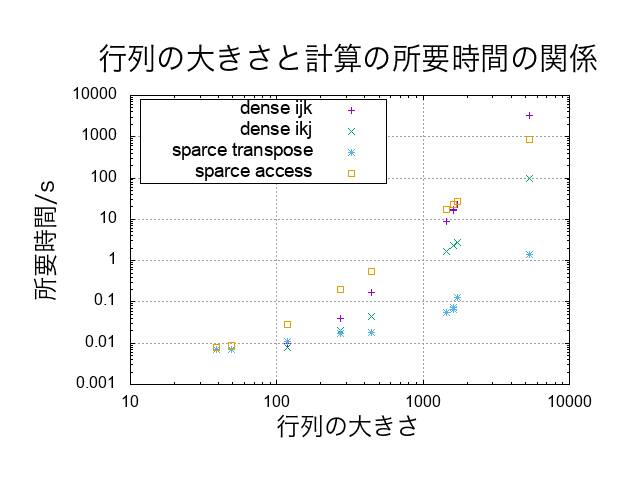
\includegraphics[width=14cm]{../graph.png}
  \caption{行列の大きさと計算の所要時間の関係}
  \end{center}
\end{figure}

ここからわかることとしては,全体として計算の速さが
sparce transpose,dense ijk,dense ikj,
sparce access
の順だということである.
また,dense ikjとsparce accessは最後の行列でだけ
順番が逆転している.

\section{考察}



\end{document}
